%%%%%%%%%%%%%%%%%%%%%%%%%%%%%%%%%%%%%%%%%%%%%%%%%%%%%%%%%%%%%%%%%%%%%%%%%%%%%%%%%%%%%%%%%%%%%%%%%%%%%%%
%%													%%
%% 	BAKALÁŘSKÁ PRÁCE -  Zásuvný modul QGIS pro pozemní monitorování radiace			%%
%% 				 Michael Kala							%%
%%													%%
%% pro formátování využita šablona: http://geo3.fsv.cvut.cz/kurzy/mod/resource/view.php?id=775 	%%
%%													%%
%%%%%%%%%%%%%%%%%%%%%%%%%%%%%%%%%%%%%%%%%%%%%%%%%%%%%%%%%%%%%%%%%%%%%%%%%%%%%%%%%%%%%%%%%%%%%%%%%%%%%%% 

\documentclass[%
  12pt,         			% Velikost základního písma je 12 bodů
  a4paper,      			% Formát papíru je A4
  oneside,       			% Oboustranný tisk
  pdftex,				    % překlad bude proveden programem 'pdftex' do PDF
%%%  draft
]{report}       			% Dokument třídy 'zpráva'
%

\newcommand{\Fbox}[1]{\fbox{\strut#1}}

\usepackage[czech, english]{babel}	% použití češtiny, angličtiny
\usepackage[utf8]{inputenc}		% Kódování zdrojových souborů je UTF8

\usepackage[square,sort,comma,numbers]{natbib}

\usepackage{caption}
\usepackage{subcaption}
\captionsetup{font=small}
\usepackage{enumitem} 
\setlist{leftmargin=*} % bez odsazení

\makeatletter
\setlength{\@fptop}{0pt}
\setlength{\@fpbot}{0pt plus 1fil}
\makeatletter

\usepackage[dvips]{graphicx}   
\usepackage{color}
\usepackage{transparent}
\usepackage{wrapfig}
\usepackage{float} 

\usepackage{cmap}           
\usepackage[T1]{fontenc}    

\usepackage{textcomp}
\usepackage[compact]{titlesec}
\usepackage{amsmath}
\addtolength{\jot}{1em} 

\usepackage{chngcntr}
\counterwithout{footnote}{chapter}

\usepackage{acronym}

\usepackage[
    unicode,                
    breaklinks=true,        
    hypertexnames=false,
    colorlinks=true, % true for print version
    citecolor=black,
    filecolor=black,
    linkcolor=black,
    urlcolor=black
]{hyperref}         

\usepackage{url}
\usepackage{fancyhdr}
%\usepackage{algorithmic}
\usepackage{algorithm}
\usepackage{algcompatible}
\renewcommand{\ALG@name}{Pseudokód}% Update algorithm name
\def\ALG@name{Pseudokód}

\usepackage[
  cvutstyle,          
  bachelor           
]{thesiscvut}


\newif\ifweb
\ifx\ifHtml\undefined % Mimo HTML.
    \webfalse
\else % V HTML.
    \webtrue
\fi 

\renewcommand{\figurename}{Obrázek}
\def\figurename{Obrázek}

%%%%%%%%%%%%%%%%%%%%%%%%%%%%%%%%%%%%%%%%%%%%%%%%%%%%%%%%%%%%%%%%%
%%%%%%%%%%% Definice informací o dokumentu  %%%%%%%%%%%%%%%%%%%%%
%%%%%%%%%%%%%%%%%%%%%%%%%%%%%%%%%%%%%%%%%%%%%%%%%%%%%%%%%%%%%%%%%

%% Název práce
\nazev{ Zásuvný modul QGIS pro pozemní monitorování radiace}
{QGIS Plugin for Ground Radiation Monitoring     }

%% Jméno a příjmení autora
\autor{Michael}{Kala}

%% Jméno a příjmení vedoucího práce včetně titulů
\garant{Ing.~Martin~Landa,~Ph.D.}

%% Označení oboru studia
\oborstudia{Geodézie, kartografie a~geoinformatika}{}

%% Označení ústavu
\ustav{Katedra geomatiky}{}

%% Rok obhajoby
\rok{2017}

%Mesic obhajoby
\mesic{červen}

%% Místo obhajoby
\misto{Praha}

%% Abstrakt
%%% ML: rozsirit, kopie zadani je pro abstrakt malo
\abstrakt 
{Abstrakt cesky}
{Abstract english}

%% Klíčová slova
\klicovaslova
{GIS, QGIS, zásuvný~modul, python}
{GIS, QGIS, plugin, python}

%%%%%%%%%%%%%%%%%%%%%%%%%%%%%%%%%%%%%%%%%%%%%%%%%%%%%%%%%%%%%%%%%%%%%%%%

%%%%%%%%%%%%%%%%%%%%%%%%%%%%%%%%%%%%%%%%%%%%%%%%%%%%%%%%%%%%%%%%%%%%%%%%
%% Nastavení polí ve Vlastnostech dokumentu PDF
%%%%%%%%%%%%%%%%%%%%%%%%%%%%%%%%%%%%%%%%%%%%%%%%%%%%%%%%%%%%%%%%%%%%%%%%
\nastavenipdf
%%%%%%%%%%%%%%%%%%%%%%%%%%%%%%%%%%%%%%%%%%%%%%%%%%%%%%%%%%%%%%%%%%%%%%%

%%% Začátek dokumentu
\begin{document}

\catcode`\-=12  % pro vypnuti aktivniho znaku '-' pouzivaneho napr. v \cline 

% aktivace záhlaví
\zahlavi

% předefinování vzhledu záhlaví
\renewcommand{\chaptermark}[1]{%
	\markboth{\MakeUppercase
	{%
	\thechapter.%
	\ #1}}{}}

% Vysázení přebalu práce
%\vytvorobalku

% Vysázení titulní stránky práce
\vytvortitulku

% Vysázení listu zadani
\stranka{}%
	{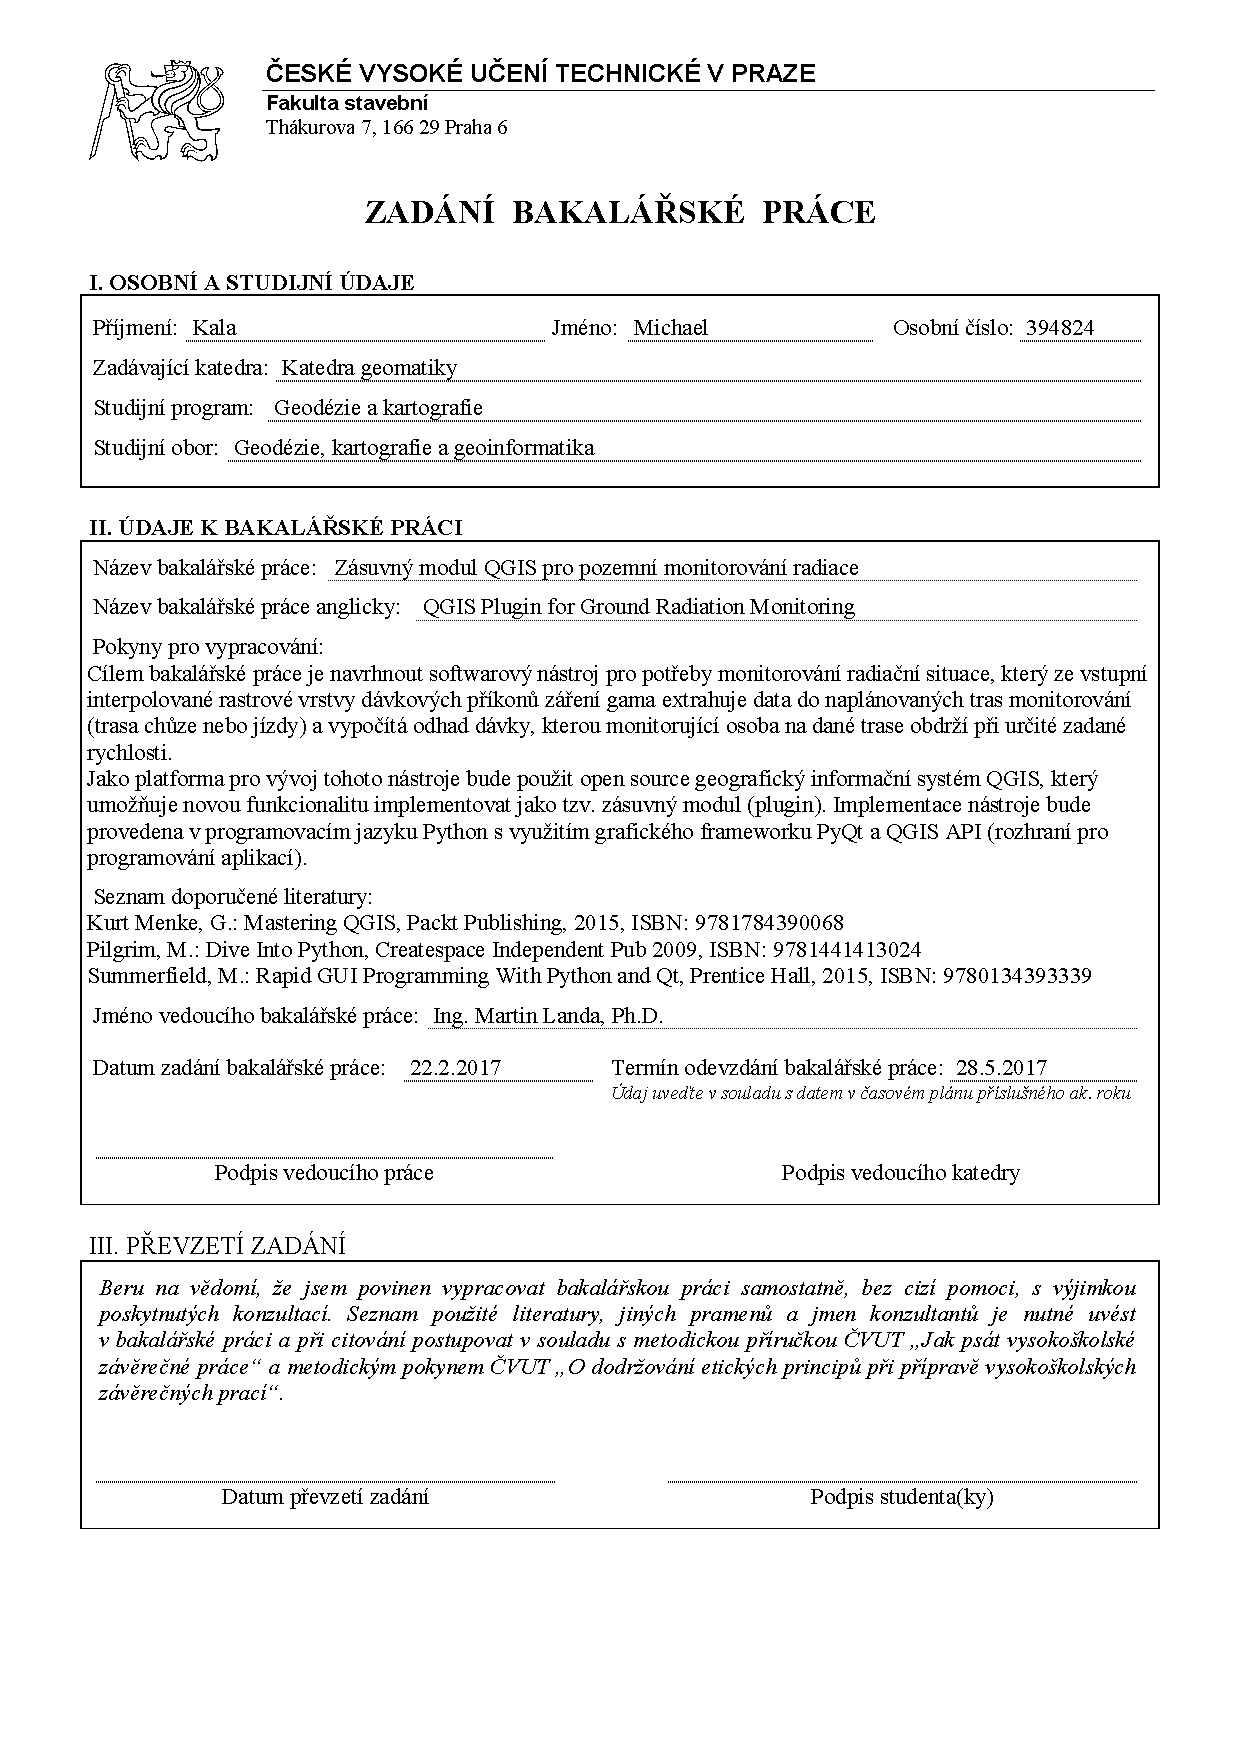
\includegraphics[scale=0.7]{./pictures/zadani.pdf}}%\sffamily\Huge\centering\ }%ZDE VLOŽIT LIST ZADÁNÍ}%
	%{\sffamily\centering Z~důvodu správného číslování stránek}

% Vysázení stránky s abstraktem
\vytvorabstrakt

% Vysázení prohlaseni o samostatnosti
\vytvorprohlaseni

% Vysázení poděkování
\stranka{%nahore
       }{%uprostred
       }{%dole
       \sffamily
	\begin{flushleft}
		\large
		\MakeUppercase{Poděkování}
	\end{flushleft}
	\vspace{1em}
		%\noindent
	\par\hspace{2ex}
	{Chtěl bych poděkovat }
}

% Vysázení obsahu
\obsah

% Vysázení seznamu obrázků
\seznamobrazku

% Vysázení seznamu tabulek
%\seznamtabulek

% jednotlivé kapitoly
\chapter{Úvod}
\label{1-uvod}
Měření veličin charakterizujících ionizující záření a studium jeho negativních dopadů, jakožto jedna z náplní práce Státního ústavu radiační ochrany, v.v.i. (\zk{SÚRO}), probíhá za účelem ochrany osob a~životního prostředí. 
Hlavní systém zjišťující radiační situaci na území České republiky se nazývá Radiační monitorovací síť (RMS). Vedle Sítě včasného zjištění (SVZ), teritoriální sítě TLD apod. jsou jednou z jejích hlavních složek také mobilní skupiny (MS) provádející pozemní monitorování radiace. \cite{suroRMS}

Cílem této bakalářské práce je implementace softwarového nástroje umožňujícího plánování optimálních tras pozemního monitorování radiace. Při únicích radioaktivních látek do ovzduší je specializovanými softwary spočtena prognóza šíření radioaktivního mraku. Jedním z produktů je také mapa dávkových příkonů záření gama pro zasaženou oblast. Vytvářený softwarový nástroj určí přibližný odhad dávky záření, kterou obdrží mobilní skupina provádějící měření na dané trase v~postiženém území. V případě překročení hraničních hodnot nástroj pomůže v~přeplánování trasy přes jiné komunikace příp. změny rychlosti jízdy vozidla tak, aby mobilní skupina nebyla vystavována nebezpečným dávkám. 
Nástroj může být hypoteticky využit také například pro havarijní plánování při navrhování tras evakuace obyvatelstva. V rámci práce je tvořena offline varianta nástroje nezbytná v případě mimořádných událostí (typu havárie jaderných elektráren), kdy nemusí být k dispozici připojení k internetu. Nicméně v budoucnu by do nástroje mohl také být implementován vlastní online plánovač tras. 

Mimo popisu vývoje nástroje se tato práce bude věnovat teoretickému základu ionizujícího záření, fyzikálním jednotkám, ve kterých je záření měřeno a počítáno, jeho biologickým účinkům na lidský organismus a metodám využívaných mobilními skupinami při pozemním monitorování. 

Nástroj je vytvářen pro \zk{SÚRO}, jako platforma pro vývoj je použit open source geografický informační systém QGIS umožňující implementaci nové funkcionality jako tzv. zásuvný modul (plugin). Nástroj je vyvíjen v programovacím jazyku Python s využitím grafického frameworku PyQt a QGIS API (rozhraní pro programování aplikací).    








% Vysázení seznamu zkratek

\begin{seznamzkratek}{ABCDE}

	\novazkratka{GNU GPL}
	      {GNU GPL}
	      {????}

	\novazkratka{SÚRO}
	      {SÚRO}
	      {Státní ústav radiační ochrany, v. v. i.}

	\novazkratka{SÚJB}
	      {SÚJB}
	      {Státní úřad pro jadernou bezpečnost}

	\novazkratka{CSV}
		  {CSV}
		  {Comma-separated values - hodnoty oddělené čárkou}
		  
	\novazkratka{KML}
		  {KML}
		  {Keyhole Markup Language}
		  
	\novazkratka{GPX}
		  {GPX}
		  {GPS Exchange Format}
	
	\novazkratka{JE}
		  {JE}
		  {Jaderná elektrárna}
		  
	\novazkratka{GIS}
		  {GIS}
		  {Grafický informační systém}
\end{seznamzkratek}

% Literatura
\nocite{*}
\def\refname{Literatura}
\bibliographystyle{mystyle}
\bibliography{literatura}


% Začátek příloh
\def\figurename{Figure}%
\prilohy

% Vysázení seznamu příloh
\seznampriloh

% Vložení souboru s přílohami
%%%%%%%%%%%%%%%%%%%%%%%%%%%%%%%%%%%%%%%%%%%%%%%%%%%%%%%%%%%%%%%%%%%%%%%%%%%%%%%%%%%
%%                 PŘÍLOHA - UŽIVATELSKÁ PŘÍRUČKA                                %%
%%%%%%%%%%%%%%%%%%%%%%%%%%%%%%%%%%%%%%%%%%%%%%%%%%%%%%%%%%%%%%%%%%%%%%%%%%%%%%%%%%%
\chapter{User guide}
\label{user-guide}

This user guide is ...

\section{Loading of plugin}
\label{plugin-load}




% Konec dokumentu
\end{document}
